\documentclass[aspectratio=169]{beamer}

% -----------------------------
% Paquetes
% -----------------------------
\usepackage[spanish]{babel}
\usepackage[utf8]{inputenc}
\usepackage[T1]{fontenc}
\usepackage{graphicx}
\graphicspath{{images/}}
\usepackage{hyperref}
\usepackage{xcolor}

% -----------------------------
% Tema (puedes cambiarlo)
% -----------------------------
\usetheme{Madrid}
\usecolortheme{default}
\setbeamertemplate{footline}{%
  \leavevmode%
  \hbox{%
  \begin{beamercolorbox}[wd=.82\paperwidth,ht=2.5ex,dp=1.2ex,leftskip=1em]{author in head/foot}%
  \end{beamercolorbox}%
  \begin{beamercolorbox}[wd=.18\paperwidth,ht=2.5ex,dp=1.2ex,rightskip=1em]{date in head/foot}%
    \hfill\insertframenumber/\inserttotalframenumber
  \end{beamercolorbox}}%
}

% -----------------------------
% Meta
% -----------------------------
\title[Token Canvas UNAB]{Cómo obtener un Token de Acceso y el ID del Curso\\en Canvas (Universidad Andrés Bello)}
\author{Guía rápida}
\date{\today}

% -----------------------------
% Helpers
% -----------------------------
\newcommand{\imgslide}[2]{%
\begin{frame}{#1}
\centering
\includegraphics[width=\linewidth,height=0.82\textheight,keepaspectratio]{#2}
\end{frame}
}

\begin{document}

% -----------------------------
% Portada
% -----------------------------
\begin{frame}
  \titlepage
\end{frame}

% -----------------------------
% Objetivo
% -----------------------------
\begin{frame}{Objetivo de esta guía}
\begin{itemize}
  \item Generar un \textbf{Token de Acceso} (Access Token) en Canvas UNAB.
  \item Copiar el \textbf{ID del Curso} desde la URL del curso.
\end{itemize}
\vspace{6pt}
\alert{Objetivo práctico:} con esta información podré subir las slides al curso.
\end{frame}

% -----------------------------
% Paso 1
% -----------------------------
\imgslide{Paso 1 — Ir a \textbf{Configuraciones}}{1_token.png}

% -----------------------------
% Paso 2
% -----------------------------
\imgslide{Paso 2 — Crear un \textbf{Nuevo token de acceso}}{2_token.png}

% -----------------------------
% Paso 3
% -----------------------------
\begin{frame}{Paso 3 — Completar el formulario del token}
\begin{columns}[T,onlytextwidth]
\column{0.54\textwidth}
\begin{block}{Qué llenar}
\begin{itemize}
  \item \textbf{Propósito:} escribe un nombre reconocible (ej.: \texttt{Curso Progra 1}).
  \item \textbf{Fecha/Hora de vencimiento:} escoge la fecha del final del semestre.
\end{itemize}
\end{block}

\begin{alertblock}{Importante}
	Si pones vencimiento y se cumple, el token muere. Y con él, tu integración. \textbf{Agrega un par de días extra a la fecha}
\end{alertblock}

\column{0.46\textwidth}
\centering
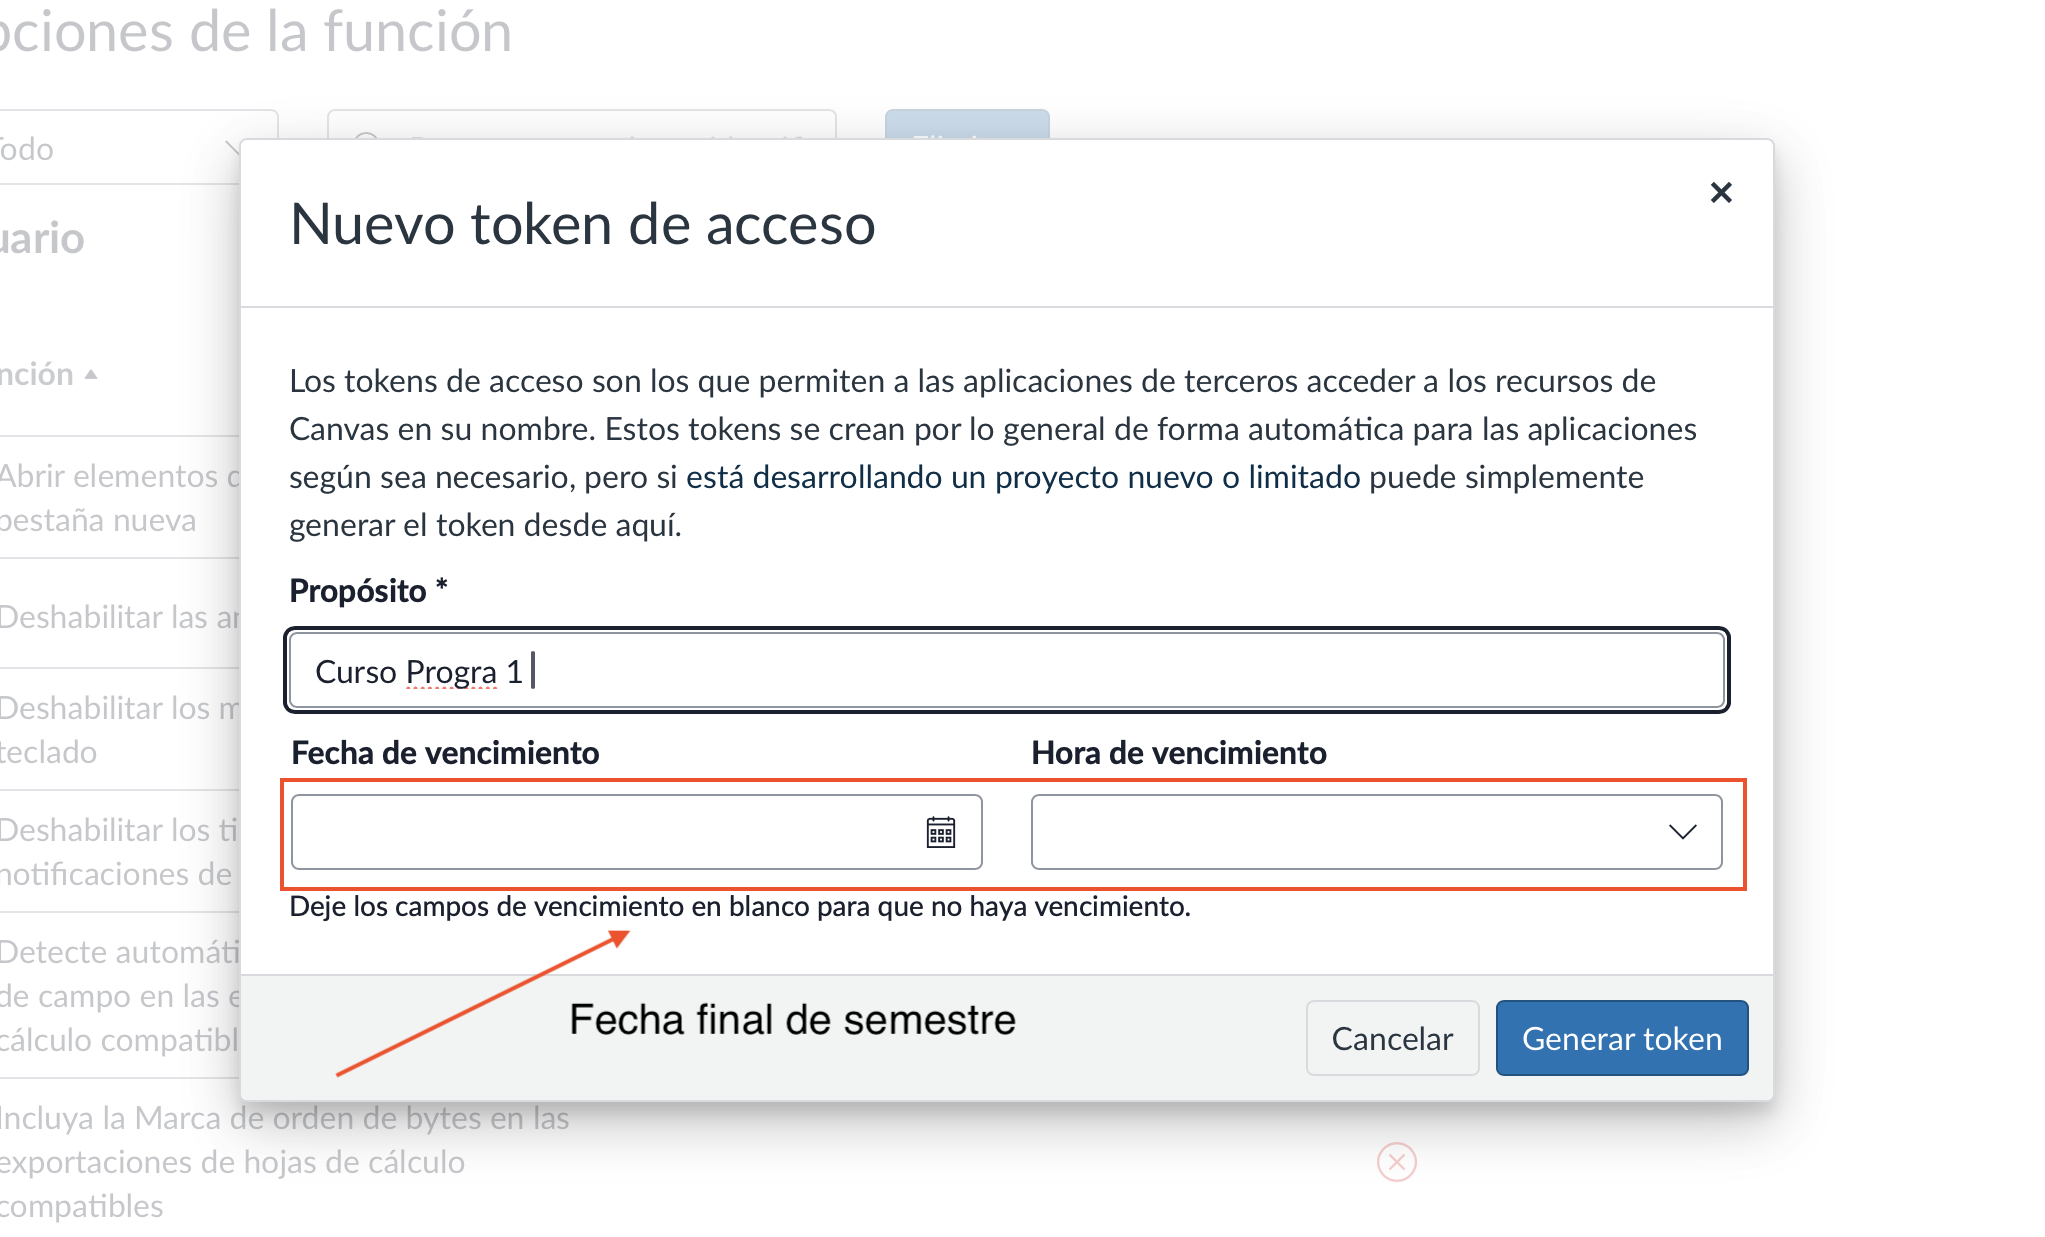
\includegraphics[width=\linewidth,height=0.78\textheight,keepaspectratio]{3_token.png}
\end{columns}
\end{frame}

% -----------------------------
% Paso 4
% -----------------------------
\imgslide{Paso 4 — Generar y \textbf{copiar el Token}}{4_token.png}

% -----------------------------
% Buenas prácticas
% -----------------------------
\begin{frame}{Buenas prácticas (para no llorar después)}
\begin{itemize}
  \item \textbf{Copia el token al instante:} Canvas suele mostrarlo completo una sola vez.
  \item \textbf{Guárdalo en un lugar seguro:} idealmente un gestor de contraseñas.
  \item Si crees que se filtró: \textbf{regenera/elimina} y usa uno nuevo.
\end{itemize}
\vspace{6pt}
\textit{Moral: token en el chat = token en el multiverso.}
\end{frame}

% -----------------------------
% ID del curso
% -----------------------------
\imgslide{Obtener el \textbf{ID del Curso} — Copiarlo desde la URL}{ID_curso.png}

% -----------------------------
% Cierre / Checklist
% -----------------------------
\begin{frame}{Checklist final}
\begin{block}{Tienes que terminar con:}
\begin{enumerate}
  \item \textbf{Access Token} (copiado para compartirlo).
  \item \textbf{Course ID} (número en la URL, ej.: \texttt{.../courses/8103}).
\end{enumerate}
\end{block}

\begin{alertblock}{Si algo falla}
Regenera el token, verifica que estés en el curso correcto y revisa permisos del usuario en Canvas.
\end{alertblock}
\end{frame}

\end{document}
